% !TEX root = main.tex

\section{Experiments}

This section will explore the same example given by the original paper, which is called ``friends and smokers'' problem. We will firstly how the definition of this example respect to the symbols we use before. Then two experiments will be deducted on knowledge base with only observed facts and knowledge base with extra rules. Finally, we will show the effects of vector length.

The experiments details are as following: total training epoch is 1000 and choose the best one according to the accuracy; for the 3.2 and 3.3, the vector length is 50. 

% !TEX root = main.tex

\subsection{Friends and Smokers}
\begin{itemize}
    \item Constant $C=C1 \cup C2=\{a,b,c,d,e,f,g,h\}\cup \{a,b,c,d,e,f,g,h\}$ is all people in two groups $C1$ and $C2$
    \item Functions: $S/1$, whether a person smokes; $F/2$, whether two persons are friends; $C/1$, whether a person have cancer.
    \item Predicate: all components of all clauses, including $F/2$, $S/1$ and $C/1$
    \item Clause: original clauses is defined as the yellow part of Figure.\ref{fig:example}. We need transfer them into disjunctive form.
\end{itemize}

The value of ``observed facts'' we know is shown in Figure.\ref{fig:example}.

\begin{figure}
    \centering
    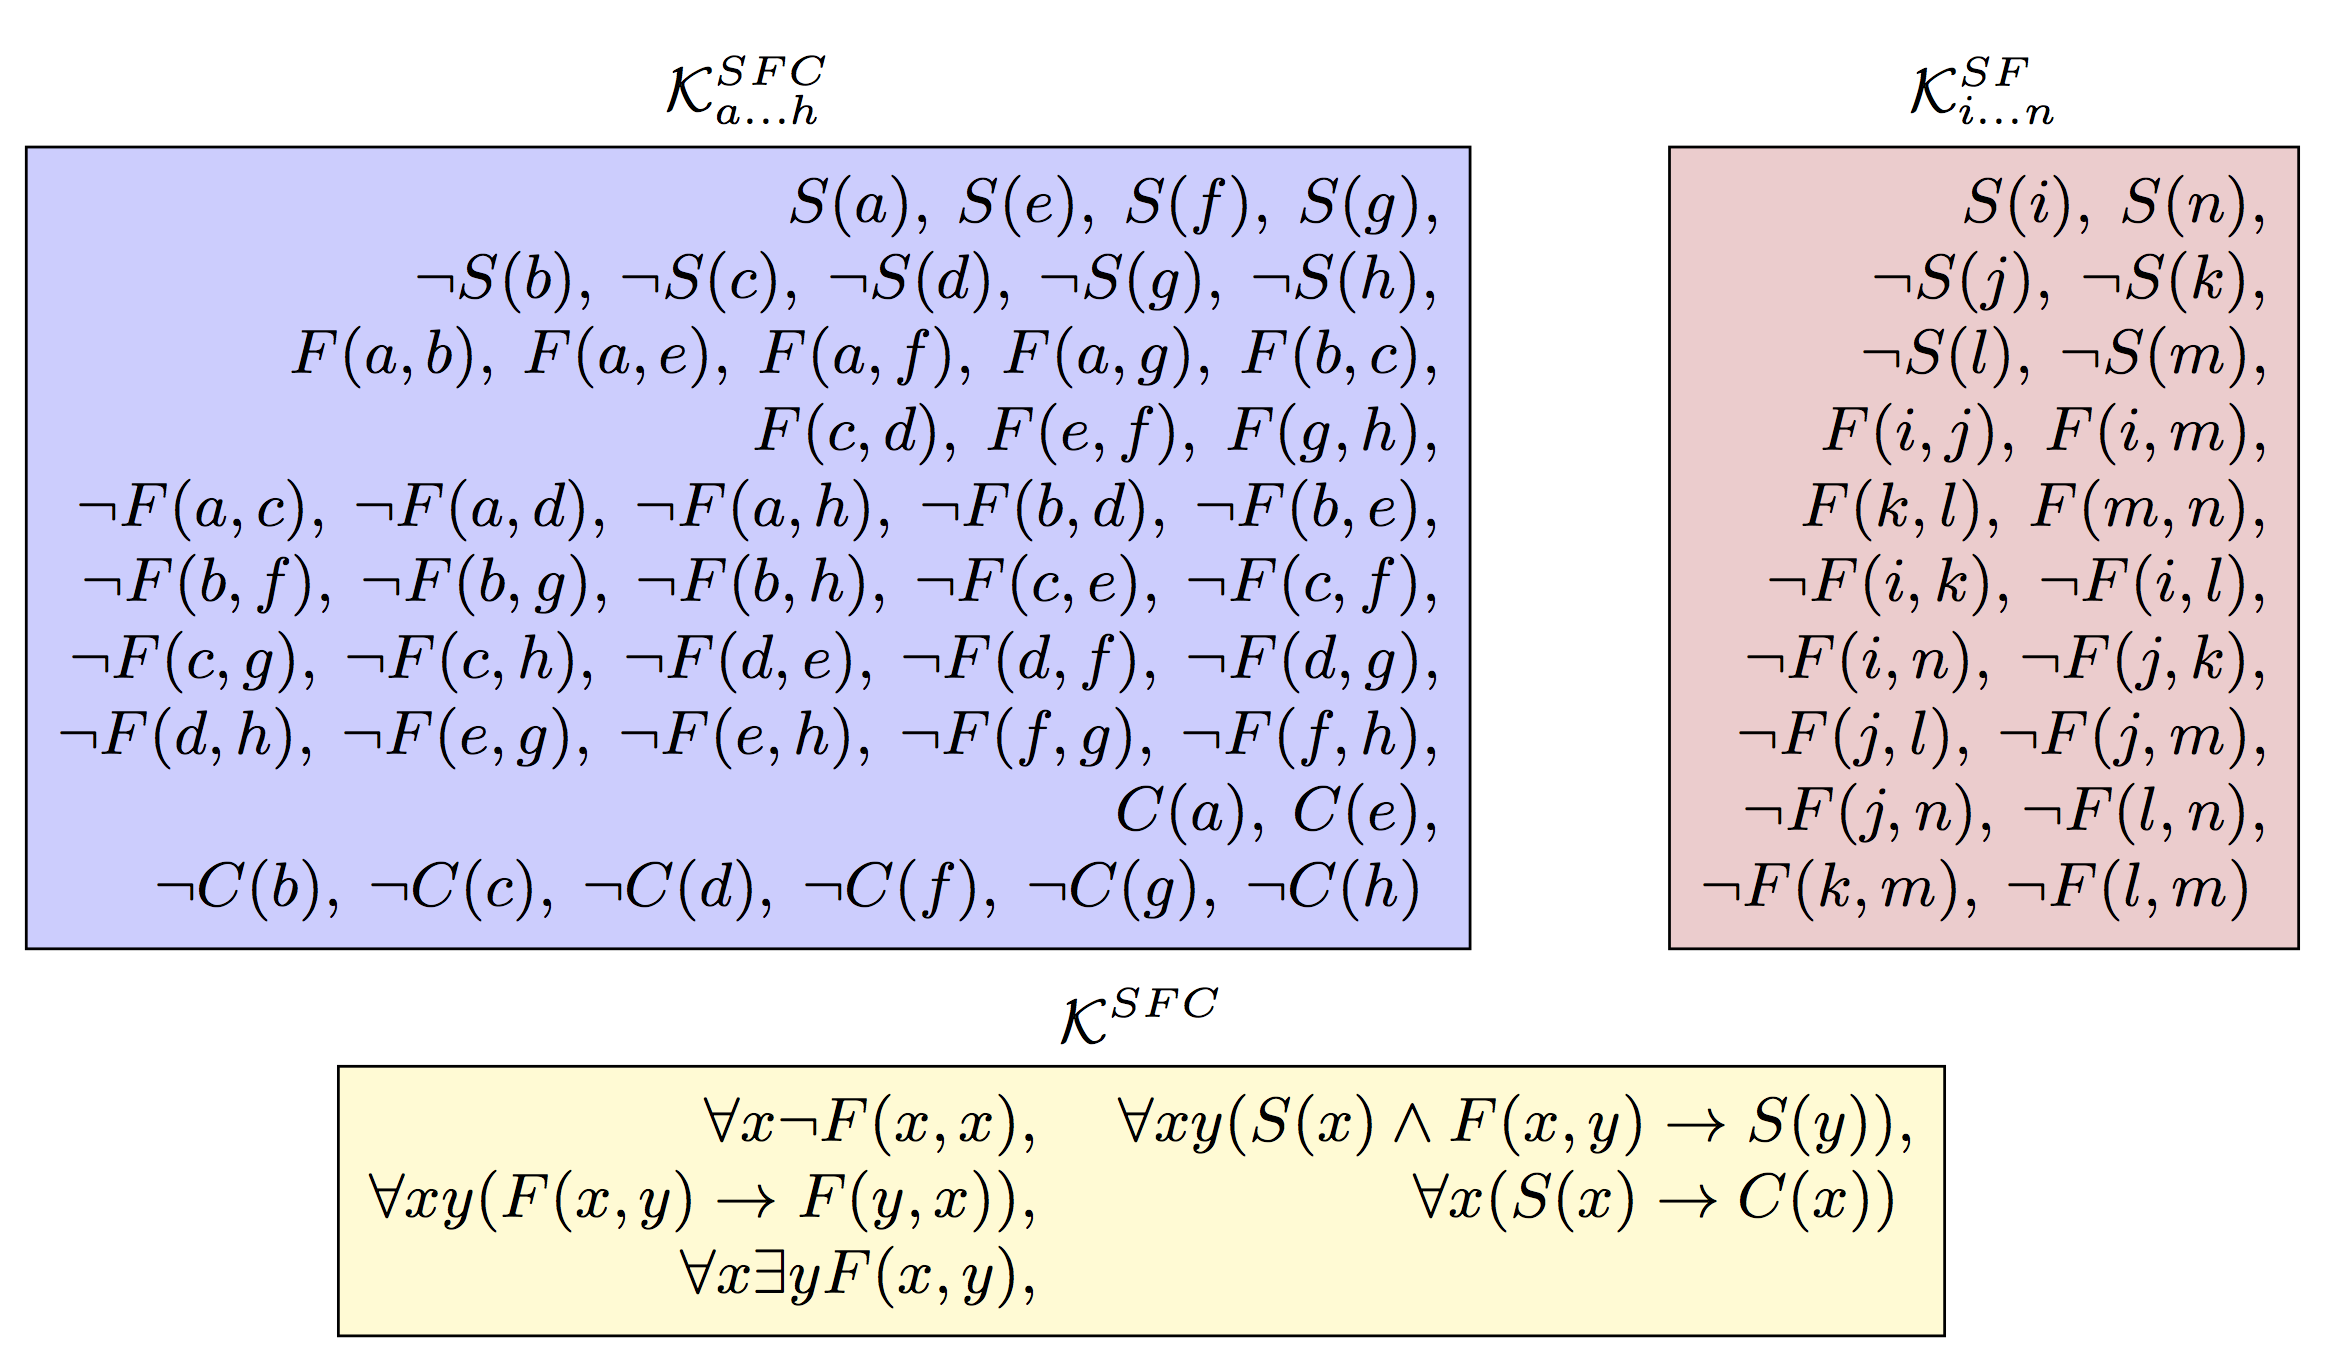
\includegraphics[width=.45\textwidth]{img/example.png}
    \caption{Friends and Smokers}
    \label{fig:example}
\end{figure}


% !TEX root = main.tex

\subsection{Fit Knowledge Base}

\begin{figure}[!]
    \centering
    % \vspace{-0.2em}
    \begin{subfigure}[]{0.24\textwidth}
        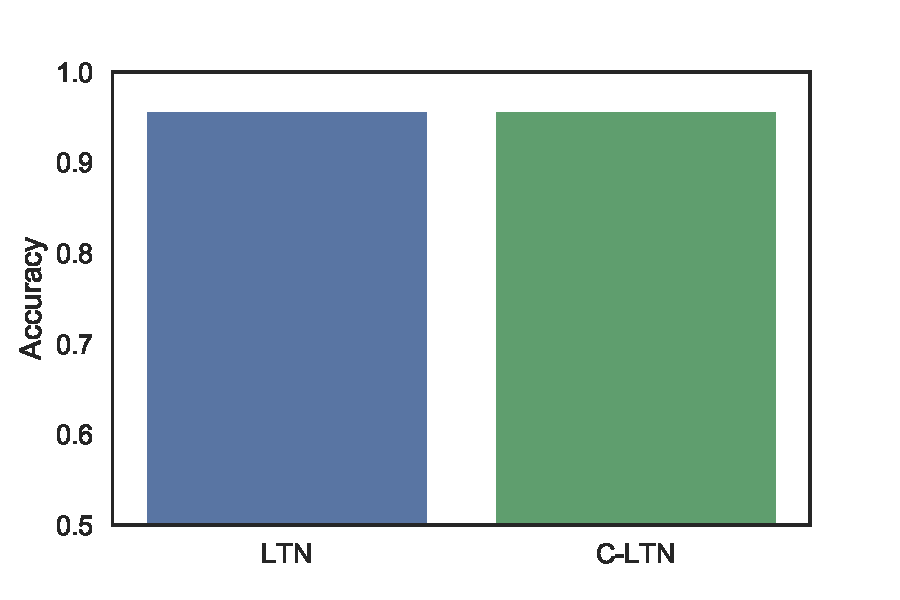
\includegraphics[width=\textwidth]{img/bar1.pdf}
        \caption{Best Accuracy on Group1}
        \label{fig:fitting-best-accuracy-1}
        %\vspace{-0.3em}
    \end{subfigure}~~~~
    \begin{subfigure}[]{0.24\textwidth}
        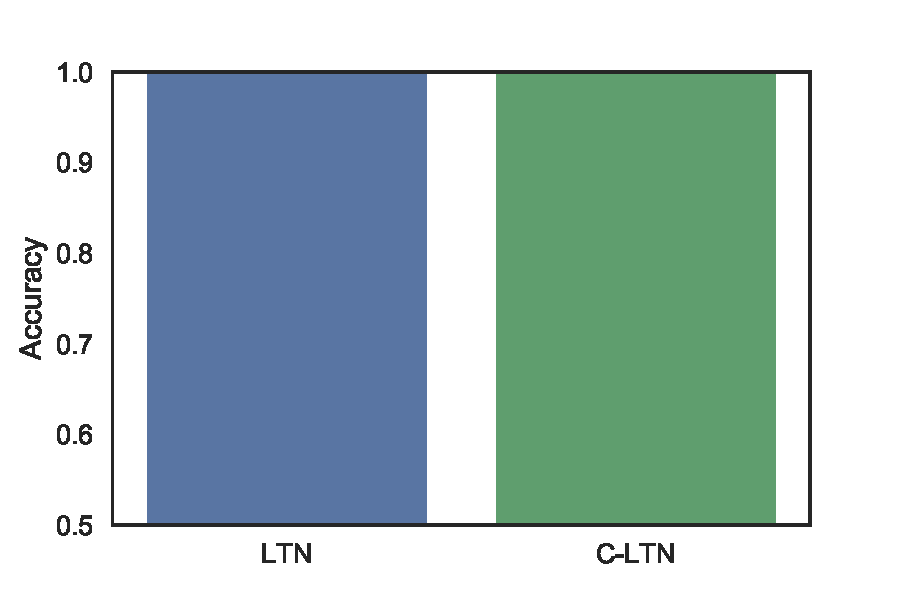
\includegraphics[width=\textwidth]{img/bar2.pdf}
        \caption{Best Accuracy on Group2}
        \label{fig:fitting-best-accuracy-2}
        %\vspace{-0.8em}
    \end{subfigure}

    \begin{subfigure}[]{0.24\textwidth}
        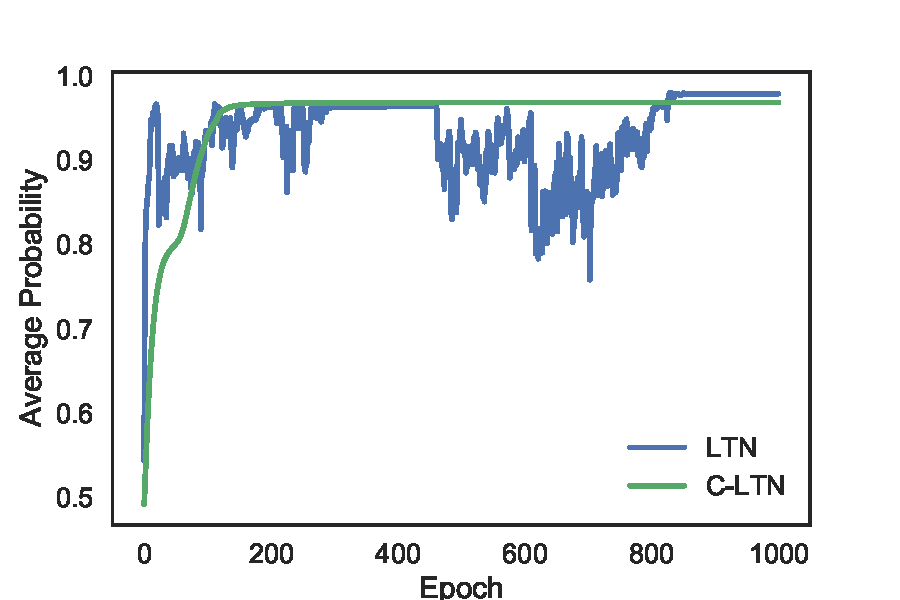
\includegraphics[width=\textwidth]{img/curve1.pdf}
        \caption{Probability w.r.t. Epoch}
        \label{fig:fitting-prob-epoch}
        %\vspace{-0.3em}
    \end{subfigure}
    \caption{Fitting Observed Facts.}
    \label{fig:fitting}
    % \vspace{-1.2em}
\end{figure}

In this experiment, we only use the oberserved facts, which is $K_{exp1} = K^{SFC}_{a \dots h} \cup K^{SF}_{i\dots n}$.

As there is no rules in this part, so we only compare the result of LTN and C-LTN.
Figure \ref{fig:fitting} shows the result of this experiment, where Figure \ref{fig:fitting-prob-epoch} is the probability change with respect to the training epoch, Figure \ref{fig:fitting-best-accuracy-1} shows the accuracy on the first group and Figure \ref{fig:fitting-best-accuracy-2} is that of the second group.

From the Figure \ref{fig:fitting}, it's clear that both LTN and C-LTN fit the observed data very well. The reason why the accuracy on first group is not $100\%$ is that there exists a contradictory pair: $S(g)$ and $\neg S(g)$. So it's not possible to make both of them $100\%$ true.

Here we also shows the fitting result for each predicate on two groups in Table \ref{table:fitting-group-1} and Table \ref{table:fitting-group-2}. And it's clear that we have a good fitting to the obseverd data.

\begin{table}[]
\centering
\begin{tabular}{c|c|c|cccccccc}
\toprule
\multirow{2}{*}{} & \multirow{2}{*}{S} & \multirow{2}{*}{C} & \multicolumn{8}{c}{F}                                 \\ \cmidrule{4-11}
                  &                    &                    & a    & b    & c    & d    & e    & f    & g    & h    \\ \midrule
a                 & 1.00               & 1.00               & 1.00 & 1.00 & 0.00 & 0.00 & 1.00 & 1.00 & 1.00 & 0.00 \\
b                 & 0.00               & 0.00               & 1.00 & 0.11 & 1.00 & 0.00 & 0.00 & 0.00 & 0.00 & 0.00 \\
c                 & 0.00               & 0.00               & 0.00 & 1.00 & 0.01 & 1.00 & 0.00 & 0.00 & 0.00 & 0.00 \\
d                 & 0.00               & 0.00               & 0.00 & 0.00 & 1.00 & 0.00 & 0.00 & 0.00 & 0.00 & 0.00 \\
e                 & 1.00               & 1.00               & 1.00 & 0.00 & 0.00 & 0.00 & 0.00 & 1.00 & 0.00 & 0.00 \\
f                 & 1.00               & 0.00               & 1.00 & 0.00 & 0.00 & 0.00 & 1.00 & 0.01 & 0.00 & 0.00 \\
g                 & 0.14               & 0.00               & 1.00 & 0.00 & 0.00 & 0.00 & 0.00 & 0.00 & 0.08 & 1.00 \\
h                 & 0.00               & 0.00               & 0.00 & 0.00 & 0.00 & 0.00 & 0.00 & 0.00 & 1.00 & 0.00 \\ \bottomrule
\end{tabular}
\caption{Fitting on Group1}
\label{table:fitting-group-1}
\end{table}

\begin{table}[]
\centering
\begin{tabular}{c|c|c|cccccc}
\toprule
\multirow{2}{*}{} & \multirow{2}{*}{S} & \multirow{2}{*}{C} & \multicolumn{6}{l}{F}                   \\ \cmidrule{4-9}
                  &                    &                    & i    & j    & k    & l    & m    & n    \\ \midrule
i                 & 1.00               & 0.05               & 0.74 & 1.00 & 0.01 & 0.01 & 1.00 & 0.00 \\
j                 & 0.00               & 0.02               & 1.00 & 0.00 & 0.00 & 0.00 & 0.00 & 0.00 \\
k                 & 0.00               & 0.09               & 0.01 & 0.00 & 0.02 & 0.90 & 0.01 & 0.03 \\
l                 & 0.00               & 0.02               & 0.01 & 0.00 & 0.90 & 0.01 & 0.01 & 0.01 \\
m                 & 0.00               & 0.11               & 1.00 & 0.00 & 0.01 & 0.01 & 0.51 & 1.00 \\
n                 & 1.00               & 0.05               & 0.00 & 0.00 & 0.03 & 0.01 & 1.00 & 0.02 \\ \bottomrule
\end{tabular}
\caption{Fitting on Group2}
\label{table:fitting-group-2}
\end{table}

Finally, in Table \ref{table:fitting-learned-rules}, we shows the reliability of the rules on this situation. Even though that we didn't use the rules in this experiments, it still got a reasonable probability for each rule.

\begin{table}[]
\centering
\begin{tabular}{lll}
\toprule
Propositional           & Group1   & Group2   \\ \midrule
$\forall \neg F(x, x)$                & 0.75     & 0.666667 \\
$\forall x y F(x,y)\rightarrow F(y,x) $      & 0.984375 & 0.944444 \\
$\forall x \exists y F(x,y) $                 & 1        & 1        \\
$\forall x y S(x) F(x,y)\rightarrow S(y) $ & 0.953125 & 0.916667 \\
$\forall x S(x)\rightarrow C(x) $            & 0.75     & 0.6666   \\ \bottomrule
\end{tabular}
\caption{Learned Rules}
\label{table:fitting-learned-rules}
\end{table}


% !TEX root = main.tex

\subsection{Learn From Rule}

\begin{figure}[!]
    \centering
    % \vspace{-0.2em}
    \begin{subfigure}[]{0.24\textwidth}
        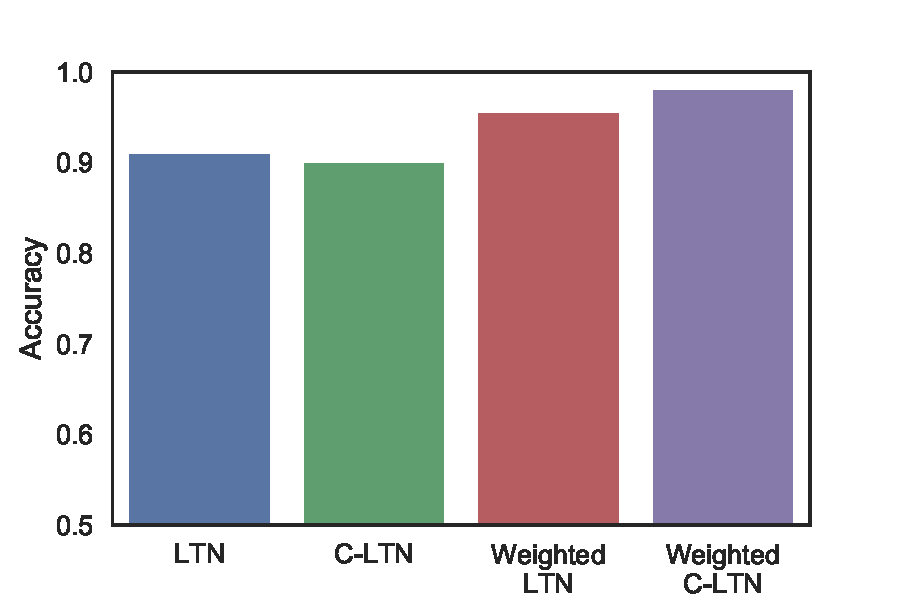
\includegraphics[width=\textwidth]{img/bar3.pdf}
        \caption{Best Accuracy on Group1}
        \label{fig:learning-best-accuracy-1}
        %\vspace{-0.3em}
    \end{subfigure}~~~~
    \begin{subfigure}[]{0.24\textwidth}
        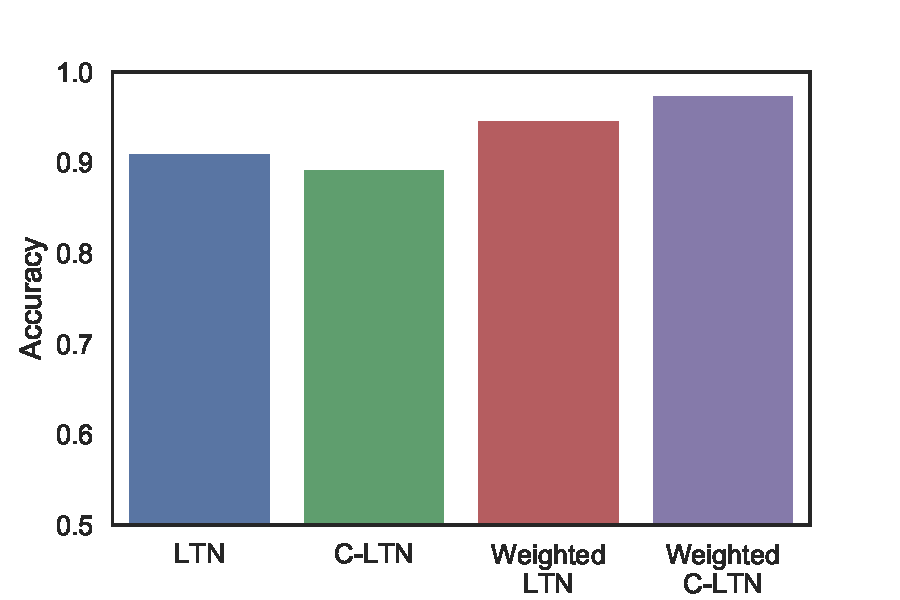
\includegraphics[width=\textwidth]{img/bar4.pdf}
        \caption{Best Accuracy on Group2}
        \label{fig:learning-best-accuracy-2}
        %\vspace{-0.8em}
    \end{subfigure}

    \begin{subfigure}[]{0.24\textwidth}
        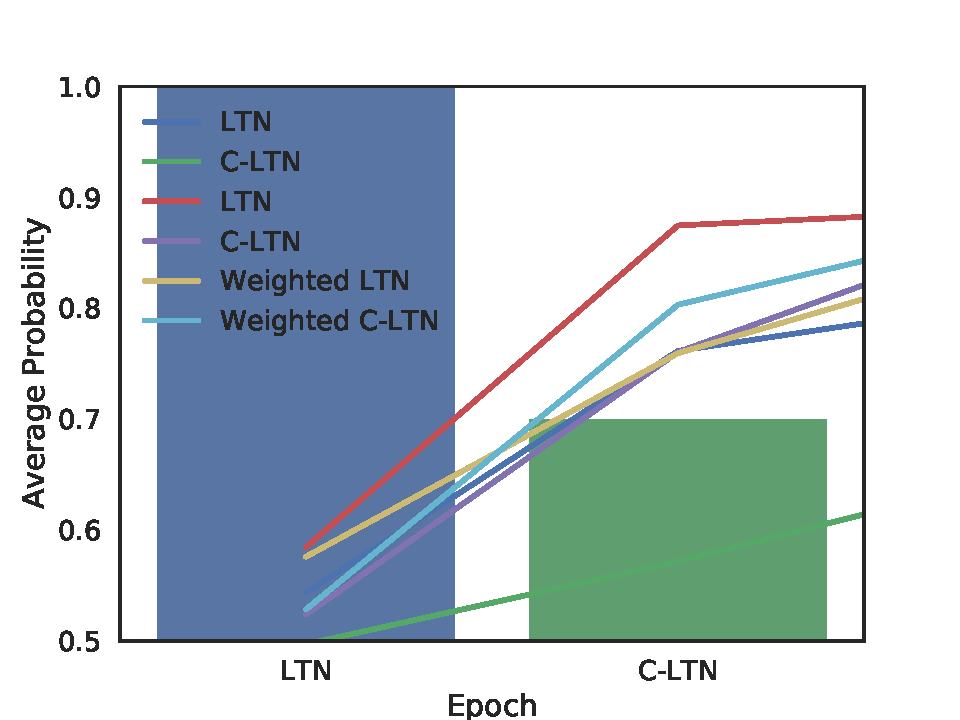
\includegraphics[width=\textwidth]{img/curve2.pdf}
        \caption{Probability w.r.t. Epoch}
        \label{fig:learning-prob-epoch}
        %\vspace{-0.3em}
    \end{subfigure}
    \caption{Learning from Observed Facts \& Rules.}
    \label{fig:learning}
    % \vspace{-1.2em}
\end{figure}

Firgure \ref{fig:learning} shows the result of two models on datasets. Like the result in last subsection, this figure containts three subfigures, including probability changes and best accuracy on two groups.

Some interesting phenomenon can be concluded from the results.

First, by comparing results on weighted and unweighted dataset, we can see that training on weighted dataset gets a better performance.
As we said before, this is because the weighted method treat each proposal as one clause, which could avoid the unbalanced training.

Second, C-LTN on weighted datasets shows the best performance. That's because CNN has better fitting ability and more stable in training.

What's more, like the last experiment, the curve of C-LTN is more smooth than that of LTN, which means the stable property of C-LTN maintains on both datasets.

Here we also shows the details of learning results in Table \ref{table:learning-group-1}, \ref{table:learning-group-2}, \ref{table:learning-learned-rules}.

\begin{table}[]
\centering
\begin{tabular}{c|c|c|cccccccc}
\toprule
\multirow{2}{*}{} & \multirow{2}{*}{S} & \multirow{2}{*}{C} & \multicolumn{8}{l}{F}                                 \\ \cmidrule{4-11}
                  &                    &                    & a    & b    & c    & d    & e    & f    & g    & h    \\ \midrule
a                 & 1.00               & 1.00               & 1.00 & 1.00 & 0.00 & 0.00 & 1.00 & 1.00 & 1.00 & 0.00 \\
b                 & 0.00               & 0.00               & 1.00 & 0.05 & 1.00 & 0.00 & 0.00 & 0.00 & 0.00 & 0.00 \\
c                 & 0.00               & 0.00               & 0.00 & 1.00 & 0.93 & 1.00 & 0.00 & 0.00 & 0.00 & 0.00 \\
d                 & 0.00               & 0.00               & 0.00 & 0.00 & 1.00 & 0.00 & 0.00 & 0.00 & 0.00 & 0.00 \\
e                 & 1.00               & 1.00               & 1.00 & 0.00 & 0.00 & 0.00 & 0.00 & 1.00 & 0.00 & 0.00 \\
f                 & 1.00               & 0.00               & 1.00 & 0.00 & 0.00 & 0.00 & 1.00 & 0.01 & 0.00 & 0.00 \\
g                 & 0.49               & 0.00               & 1.00 & 0.00 & 0.00 & 0.00 & 0.00 & 0.00 & 0.10 & 1.00 \\
h                 & 0.00               & 0.00               & 0.00 & 0.00 & 0.00 & 0.00 & 0.00 & 0.00 & 1.00 & 0.00 \\ \bottomrule
\end{tabular}
\caption{Fitting and Learning on Group1}
\label{table:learning-group-1}
\end{table}

\begin{table}[]
\centering
\begin{tabular}{c|c|c|cccccc}
\toprule
\multirow{2}{*}{} & \multirow{2}{*}{S} & \multirow{2}{*}{C} & \multicolumn{6}{l}{F}                   \\ \cmidrule{4-9}
                  &                    &                    & i    & j    & k    & l    & m    & n    \\ \midrule
i                 & 1.00               & 0.84               & 0.13 & 1.00 & 0.00 & 0.00 & 1.00 & 0.00 \\
j                 & 0.00               & 0.25               & 1.00 & 0.00 & 0.00 & 0.00 & 0.00 & 0.00 \\
k                 & 0.00               & 0.76               & 0.00 & 0.00 & 0.13 & 1.00 & 0.00 & 0.03 \\
l                 & 0.00               & 0.08               & 0.00 & 0.00 & 1.00 & 0.05 & 0.00 & 0.00 \\
m                 & 0.00               & 0.54               & 1.00 & 0.00 & 0.00 & 0.00 & 0.32 & 1.00 \\
n                 & 1.00               & 0.04               & 0.00 & 0.00 & 0.03 & 0.00 & 1.00 & 0.05 \\ \bottomrule
\end{tabular}
\caption{Fitting and Learning on Group2}
\label{table:learning-group-2}
\end{table}

\begin{table}[]
\centering
\begin{tabular}{lll}
\toprule
Propositional           & Group1   & Group2   \\ \midrule
$\forall \neg F(x, x)$                & 0.625    & 0.5      \\
$\forall x y F(x,y)\rightarrow F(y,x) $      & 0.984375 & 0.916667 \\
$\forall x \exists y F(x,y) $                 & 1        & 1        \\
$\forall x y S(x) F(x,y)\rightarrow S(y) $ & 0.9375   & 0.916667 \\
$\forall x S(x)\rightarrow C(x) $            & 0.75     & 0.666667 \\ \bottomrule
\end{tabular}
\caption{Learned Rules}
\label{table:learning-learned-rules}
\end{table}


% !TEX root = main.tex

\subsection{Parameter Sensitive}

\begin{figure}[!]
    \centering
    % \vspace{-0.2em}
    \begin{subfigure}[]{0.23\textwidth}
        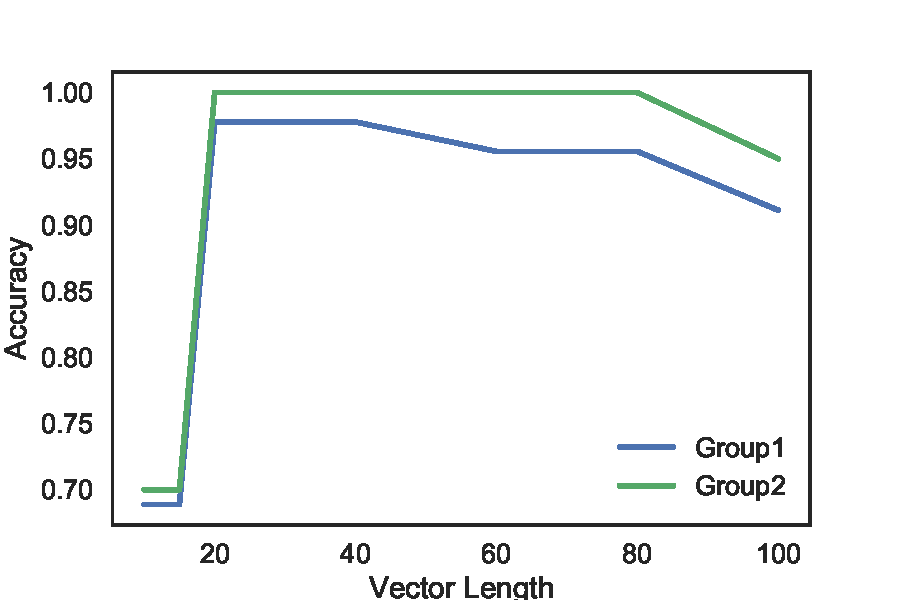
\includegraphics[width=\textwidth]{img/curve3.pdf}
        \caption{Fitting Observed Facts}
        \label{fig:sensitive-best-accuracy-1}
        %\vspace{-0.3em}
    \end{subfigure}
    \begin{subfigure}[]{0.23\textwidth}
        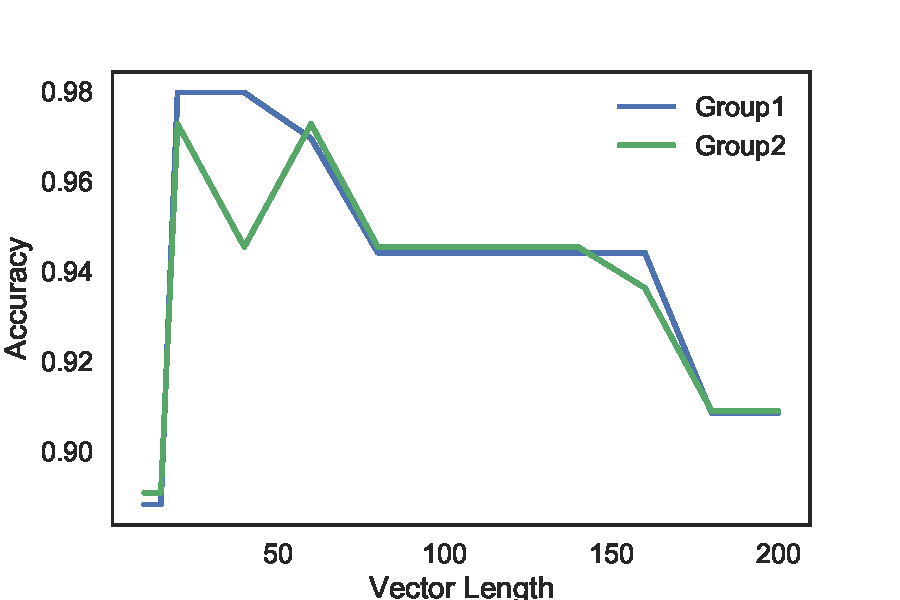
\includegraphics[width=\textwidth]{img/curve4.pdf}
        \caption{Learning from Rules }
        \label{fig:sensitive-best-accuracy-2}
        %\vspace{-0.3em}
    \end{subfigure}
    \caption{Best Accuracy w.r.t. Vector Length.}
    \label{fig:sensitive}
    % \vspace{-1.2em}
\end{figure}


In this part, we want to test the effect of vector length $k$. We enumerate the vector length from 1 to 100 and shows the best accuracy on two groups. We did our experiments on both observed data and weighted dataset with rule. As the performance of C-LNT is better than LNT, we only shows the result of C-LNT, which is shown in Figure \ref{fig:sensitive}.

Figure \ref{fig:fitting-best-accuracy-1} shows the result in observed dataset.
From this figure, we can conclude that the performance is not always getting better with the increase of vector length. Actually, it's getting worse when $k$ is too big. That's may because the under training problem. That is, as we increase the vector length, we may need to repeat more to get a good model. Those effors is unnecessary because we would get a good result when $k \in [20,40]$.

